\section{Protocols}
\subsection{Sequencer}
This protocol ensures that N producers fire in a cyclic sequence.\\

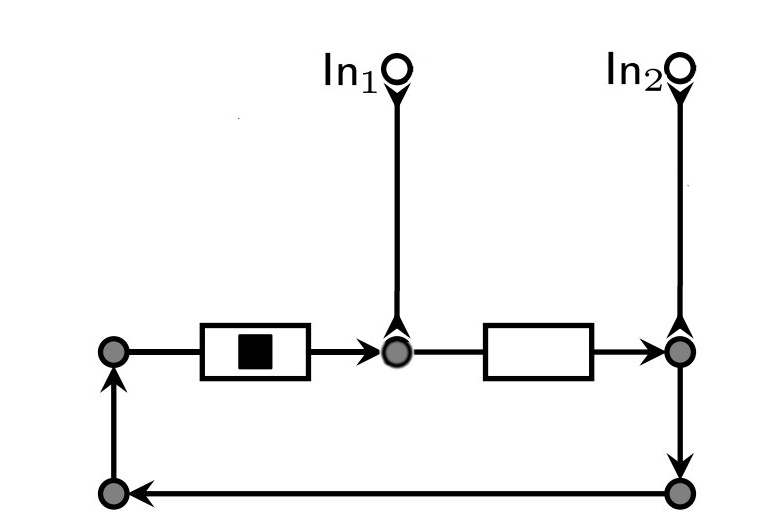
\includegraphics[]{img/seq.png}\\
%
It has the following data stream semantics:\\
%
$
\vspace{0.2cm}\sequencer (\langle \alpha_0, a_0 \rangle, \langle \alpha_1, a_1 \rangle,\;...\; \langle \alpha_{\textbf{N}-1}, a_{\textbf{N}-1} \rangle) \equiv \\
\vspace{0.2cm}\hphantom \qquad  \alpha_0(0) < \alpha_1(0) < ... < \alpha_{\textbf{N}-1}(0) < \alpha_0(1) \\
\hphantom \qquad \sequencer(\langle \alpha_0', a_0' \rangle, \langle \alpha_1', a_1' \rangle,\;...\; \langle \alpha_{N-1}', a_{\textbf{N}-1}' \rangle)
$


\subsection{Alternator}
This protocol waits for all N inputs to put and the one output to get, after which the data of the first producer is instantly consumed.
All the other producers have their output buffered, and consumed one by one in a set order.
Only after all data has been consumed, may the producers fire again.\\

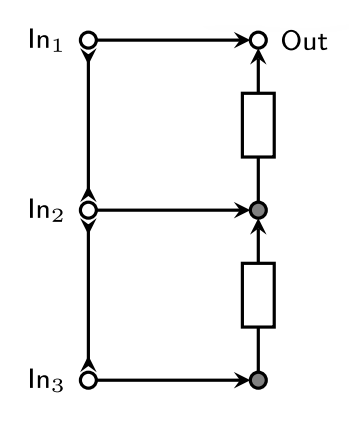
\includegraphics[]{img/alt.png}\\
%
It has the following data stream semantics:\\
%
$
\vspace{0.2cm} \alternator (\langle \alpha_0, a_0 \rangle, \langle \alpha_1, a_1 \rangle,\; ... \; \langle \alpha_{\textbf{N}-1}, a_{\textbf{N}-1} \rangle; \langle \beta, b \rangle) \equiv\\
\vspace{0.2cm} \hphantom \qquad \alpha_0(0) = \alpha_1(0) = ... = \alpha_{\textbf{N}-1}(0) = \beta(0) < \beta(1) < ... < \beta(\textbf{N}-1) < \alpha_0(1) \\
\vspace{0.2cm} \hphantom \qquad\forall 0 \leq i < \textbf{N} :\quad b(i) = a_i(0) \\
\hphantom \qquad \alternator (\langle \alpha_0', a_0' \rangle, \langle \alpha_1', a_1' \rangle,\;...\; \langle \alpha_{N-1}', a_{N-1}' \rangle; \langle \beta(\textbf{N},\;...), b(\textbf{N},\;...) \rangle)
$

\subsection{Early Async Replicator}
This protocol has one producer, whose data is buffered when put, and $N$ consumers, which all replicate the producers data.
All consumers fire simultaneously, but strictly after the producer.\\

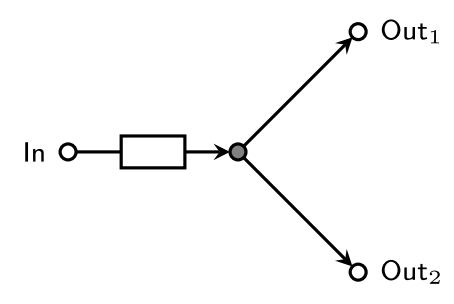
\includegraphics[]{img/EARep.png}\\
%
It has the following data stream semantics:\\
%
$
\vspace{0.2cm}\earep (\langle \alpha, a \rangle ; \langle \beta_0, b_0 \rangle, \langle \beta_1, b_1 \rangle,\; ... \; \langle \beta_{\textbf{N}-1}, b_{\textbf{N}-1} \rangle) \equiv \\
\vspace{0.2cm} \hphantom \qquad \forall 0 \leq i < \textbf{N} : \quad \alpha(0) < \beta_i(0) < \alpha(1) \land a(0) = b_i(0) \\
\hphantom \qquad\forall 0 \leq i < \textbf{N} :\quad \forall 0 \leq i < \textbf{N} : \beta_i(0) = \beta_j(0)
$\\

\subsection{Early Async Out Sequencer}
Given one producer and multiple consumers, this protocol saves a production to a buffer and then directs it to one consumer. The consumer which receives the message changes for each production, visiting every consumer in a predefined sequence.\\

\includegraphics[]{img/EAOSeq.png}\\
%
It has the following data stream semantics:\\
%
$
\vspace{0.2cm}\eaoseq (\langle \alpha, a \rangle;\langle \beta_0, b_0 \rangle, \langle \beta_1, b_1 \rangle,\;...\; \langle \beta_{\textbf{N}-1}, b_{\textbf{N}-1} \rangle) \equiv \\
\vspace{0.2cm} \hphantom \qquad \alpha(0) < \beta_0(0) < \alpha(1) \land a(0) = b_0(0) \\
\vspace{0.2cm} \hphantom \qquad \eaoseq (\langle \alpha', a' \rangle; \langle \beta_1, b_1 \rangle,\langle \beta_2, b_2 \rangle,\;...\; \langle \beta_{\textbf{N}-1}, b_{\textbf{N}-1} \rangle, \langle \beta_0', b_0' \rangle)
$
